\documentclass[12pt]{article}

\usepackage{amsmath, mathtools}
\usepackage{amsfonts}
\usepackage{amssymb}
\usepackage{graphicx}
\usepackage{colortbl}
\usepackage{xr}
\usepackage{hyperref}
\usepackage{longtable}
\usepackage{xfrac}
\usepackage{tabularx}
\usepackage{float}
\usepackage{siunitx}
\usepackage{booktabs}
\usepackage{caption}
\usepackage{pdflscape}
\usepackage{afterpage}

\usepackage[round]{natbib}

%\usepackage{refcheck}

\hypersetup{
    bookmarks=true,         % show bookmarks bar?
      colorlinks=true,       % false: boxed links; true: colored links
    linkcolor=red,          % color of internal links (change box color with 
%linkbordercolor)
    citecolor=green,        % color of links to bibliography
    filecolor=magenta,      % color of file links
    urlcolor=cyan           % color of external links
}

%% Comments

\usepackage{color}

\newif\ifcomments\commentstrue

\ifcomments
\newcommand{\authornote}[3]{\textcolor{#1}{[#3 ---#2]}}
\newcommand{\todo}[1]{\textcolor{red}{[TODO: #1]}}
\else
\newcommand{\authornote}[3]{}
\newcommand{\todo}[1]{}
\fi

\newcommand{\wss}[1]{\authornote{blue}{SS}{#1}} 
\newcommand{\plt}[1]{\authornote{magenta}{TPLT}{#1}} %For explanation of the template
\newcommand{\an}[1]{\authornote{cyan}{Author}{#1}}

%% Common Parts

\newcommand{\progname}{Diagnose} % PUT YOUR PROGRAM NAME HERE %Every program
                                % should have a name


% For easy change of table widths
\newcommand{\colZwidth}{1.0\textwidth}
\newcommand{\colAwidth}{0.13\textwidth}
\newcommand{\colBwidth}{0.82\textwidth}
\newcommand{\colCwidth}{0.1\textwidth}
\newcommand{\colDwidth}{0.05\textwidth}
\newcommand{\colEwidth}{0.8\textwidth}
\newcommand{\colFwidth}{0.17\textwidth}
\newcommand{\colGwidth}{0.5\textwidth}
\newcommand{\colHwidth}{0.28\textwidth}

% Used so that cross-references have a meaningful prefix 
\newcounter{defnum} %Definition Number
\newcommand{\dthedefnum}{GD\thedefnum}
\newcommand{\dref}[1]{GD\ref{#1}}
\newcounter{datadefnum} %Datadefinition Number
\newcommand{\ddthedatadefnum}{DD\thedatadefnum}
\newcommand{\ddref}[1]{DD\ref{#1}}
\newcounter{theorynum} %Theory Number
\newcommand{\tthetheorynum}{T\thetheorynum}
\newcommand{\tref}[1]{T\ref{#1}}
\newcounter{tablenum} %Table Number
\newcommand{\tbthetablenum}{T\thetablenum}
\newcommand{\tbref}[1]{TB\ref{#1}}
\newcounter{assumpnum} %Assumption Number
\newcommand{\atheassumpnum}{P\theassumpnum}
\newcommand{\aref}[1]{A\ref{#1}}
\newcounter{goalnum} %Goal Number
\newcommand{\gthegoalnum}{P\thegoalnum}
\newcommand{\gsref}[1]{GS\ref{#1}}
\newcounter{instnum} %Instance Number
\newcommand{\itheinstnum}{IM\theinstnum}
\newcommand{\iref}[1]{IM\ref{#1}}
\newcounter{reqnum} %Requirement Number
\newcommand{\rthereqnum}{P\thereqnum}
\newcommand{\rref}[1]{R\ref{#1}}
\newcounter{nreqnum} %NRequirement Number
\newcommand{\nrthereqnum}{NP\thenreqnum}
\newcommand{\nrref}[1]{NR\nref{#1}}
\newcounter{lcnum} %Likely change number
\newcommand{\lthelcnum}{LC\thelcnum}
\newcommand{\lcref}[1]{LC\ref{#1}}
\newcounter{ucnum} %Likely change number
\newcommand{\ltheucnum}{UC\thelcnum}
\newcommand{\ucref}[1]{UC\ref{#1}}

\begin{document}

\title{Software Requirements Specification for \progname: Medical Prediction 
Tool for Acquired immunodeficiency syndrome (AIDS)} 
\author{Andrea Clemeno}
\date{\today}
	
\maketitle

~\newpage

\pagenumbering{roman}

\tableofcontents

~\newpage

\section*{Revision History}

\begin{tabularx}{\textwidth}{p{3cm}p{2cm}X}
\toprule {\bf Date} & {\bf Version} & {\bf Notes}\\
\midrule
October 10 2020 & 1.0 & Initial Draft of SRS\\
December 3 & 1.1 & Revised Draft of SRS\\
December 8 & 1.2 & 2nd Revised Draft of SRS\\
\bottomrule
\end{tabularx}

~\newpage

\section{Reference Material}

This section records information for easy reference.

\subsection{Table of Units}

Throughout this document SI (Syst\`{e}me International d'Unit\'{e}s) is employed
as the unit system. For each unit, the symbol is given followed by a
description of the unit and the name.

\renewcommand{\arraystretch}{1.2}
\begin{table}[h!]
\begin{center}
 \noindent \begin{tabular}{l l l}
    \toprule		
    \textbf{symbol} & \textbf{unit} & \textbf{name}\\
    \midrule 
    \si{\day} & time & day\\
    mL & volume	& millilitre\\
    \si{\mole} & amount of substance & mole\\
    \bottomrule
  \end{tabular}
  \end{center}
  	\caption{Table of Units}
\end{table}

 
~\newpage
\subsection{Table of Symbols}

The table that follows summarizes the symbols used in this document along with
their units. The symbols are listed in alphabetical order.

\begin{table}[H]
\renewcommand{\arraystretch}{1.2}
%\noindent \begin{tabularx}{1.0\textwidth}{l l X}
\noindent \begin{longtable*}{l l p{12cm}} \toprule
\textbf{symbol} & \textbf{unit} & \textbf{description}\\
\midrule 
$k$ & $d^{-1}$ & Elimination Constant
\\
$N$ & \si[per-mode=symbol]{\dfrac{\mol}{\mL}} & Viral Load
\\ 
$N_{o}$ & \si[per-mode=symbol]{\dfrac{\mol}{\mL}} & Initial Viral Load
\\ 
$N_{p}$ & \si[per-mode=symbol]{\dfrac{\mol}{\mL}} & Predicted Viral Load at time 
$t_{p}$
\\ 
$N_{t}$ & \si[per-mode=symbol]{\dfrac{\mol}{\mL}} & Viral Load at time $t_{t}$
\\ 
$n$ & \si[per-mode=symbol]{\mol} & Number of virions
\\ 
$r$ & \si[per-mode=symbol] {\dfrac{\mol}{mL*d}} & Rate of change of the viral 
load
\\
$t$ & \si[per-mode=symbol] {\day} & Time
\\

$t_{p}$ & \si[per-mode=symbol] {\second} & Time duration of chosen prediction 
period 
\\
$t_{t}$ & \si[per-mode=symbol] {\second} & Time duration between initial and  
secondary viral load test
\\
$V$ & \si[per-mode=symbol] {\mL} & Volume
\\
&\\
\bottomrule

\end{longtable*}
\caption{Table of Symbols}
\end{table}

\newpage

\subsection{Abbreviations and Acronyms}

The table that follows summarizes the symbols used in this document that allude 
to different sections of the Software Requirements Specification. The symbols 
are listed in alphabetical order.
\begin{table}[h!]
\begin{center}
\renewcommand{\arraystretch}{1.2}
\begin{tabular}{l l} 
  \toprule		
  \textbf{symbol} & \textbf{description}\\
  \midrule 
  A & Assumption\\
  DD & Data Definition\\
  GD & General Definition\\
  GS & Goal Statement\\
  IM & Instance Model\\
  LC & Likely Change\\
  PS & Physical System Description\\
  R & Requirement\\
  SRS & Software Requirements Specification\\
  \progname{} & Medical Diagnosis Prediction Tool\\
  & for Acquired immunodeficiency syndrome (AIDS)\\
  T & Theoretical Model\\
  ULC & Unlikely Change\\
  \bottomrule
\end{tabular}\\
\end{center}
\caption{Table of Abbreviations and Acronyms}

\end{table}

\newpage

\pagenumbering{arabic}


\section{Introduction}

Human immunodeficiency virus 1 (HIV -1) is the most common type of HIV virus 
that attacks cells of the immune system needed to fight off diseases. After 
being infected with the HIV-1 virus, the state of a patient's health worsens and 
the 
condition can be classified as Acquired immunodeficiency syndrome (AIDs), a 
disease which affects 38 million people worldwide \citep{who}. Although there is 
no cure for 
AIDs, antiretroviral 
therapy helps control a patient's condition. Having a program that assesses the 
efficient of a patient's immune system and predict their viral load progression 
will be 
useful in creating a treatment plan. The program documented here is called 
Diagnose.

The following section provides an overview of the Software Requirements 
Specification (SRS) for Diagnose. This section explains the purpose of 
this document, the scope of the requirements, the characteristics of the 
intended reader, and the organization of the document.



\subsection{Purpose of Document}

The main purpose of this document is to outline the software requirements of the 
medical prediction system. Different aspects of the system including goals, 
assumptions, theoretical models, and definitions will be explained to ensure 
full understanding of the system. The following SRS document will remain 
abstract exploring what is being solved rather than how it will be solved.

This initial document is the start of a series of documents that will 
outline the development of the software tool, \progname{}. The SRS will 
describe the system context and constraints, the specific problem definition and 
solution characteristics, requirements and likely and unlikely changes for the 
development of the tool.


\subsection{Scope of Requirements} 

The scope of the requirements includes the analysis of the HIV-1 viral load 
concentration 
over time after the viremia peak of the initial infection without the influence 
of external factors that can affect the efficiency of the immune system.



\subsection{Characteristics of Intended Reader} \label{sec_IntendedReader}

Reviewers of this documentation should have a basic understanding of virus 
dynamics and high school differential calculus. The users of \progname{} must 
have a 
higher level of expertise, as explained in Section: User Characteristics
(Section~\ref{SecUserCharacteristics}). 



\subsection{Organization of Document}

The organization of the document will present the system's goals, theories, 
definitions, and assumptions. The template for an SRS for scientific computing 
will be followed. To approach \progname{} from a higher level to a more 
elaborate level, readers can begin with reading the system's goal statements. 
Subsequently, the theoretical models will elaborate on the goal statements. 
Lastly, 
readers can finish with a more  understanding of the system by reading instance 
models of the system. 

Oppositely, readers can read from the instance models to the goal statements for 
a more specific to general understanding.




\section{General System Description}

This section provides general information about the system. It identifies 
the interfaces
between the system and its environment, describes the user characteristics, and 
lists the
system constraints.


\subsection{System Context}

The flow chart in (Figure~\ref{Fig_SystemContext}) shows the system 
context. The circles 
represent a user that interacts with the software. The rectangle represents the 
software system (\progname{}). The arrows display the input data from the 
user 
and the output data that is useful for the user. The interaction presented will 
be facilitated using an application programming interface (API).


\begin{figure}[ht]
\begin{center}
 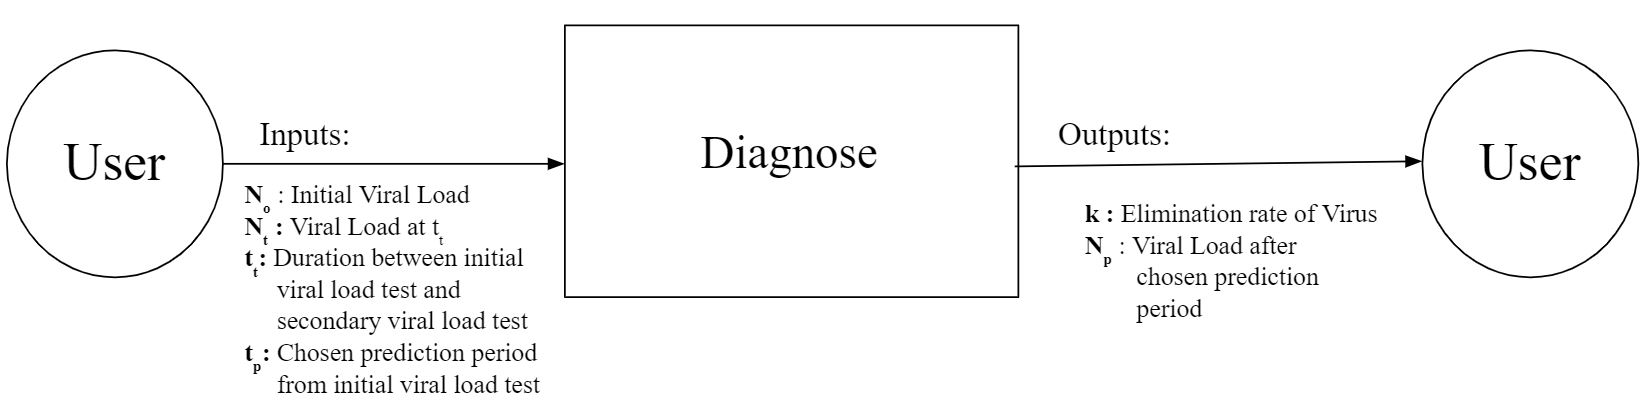
\includegraphics[width=1\textwidth]{systemcontext.jpg}
\caption{System Context}
\label{Fig_SystemContext} 
\end{center}
\end{figure}

\begin{itemize}
\item User Responsibilities:
\begin{itemize}
\item Provide viral load data for patient's initial and secondary viral load 
tests, time duration between the tests and the time duration between the initial 
test and the chosen prediction date.
\item Ensure required software assumptions (Section~\ref{sec_assumpt}) are 
appropriate for any particular problem the software addresses.

\end{itemize}
\item \progname{} Responsibilities:
\begin{itemize}
\item Assess the input data and determine if the required physical and software 
constraints (Section~\ref{sec_DataConstraints}) are met.
\item Calculate the elimination rate of the virus and the predicted viral load 
after the chosen prediction period.
\end{itemize}
\end{itemize}

\subsection{User Characteristics} \label{SecUserCharacteristics}
The users of \progname{} should be HIV healthcare providers including 
doctors of medicine (MD) or doctors of osteopathic medicine (DO), nurse 
practitioners (NP), or a physician assistant (PA). \citep{cdc}


\subsection{System Constraints} \label{Sec_constraints}

The system, \progname{}, is limited to only instances where viral load 
is eliminating. If 
the viral load is increasing, the immune system has not recognized the intruders 
and a estimation of immune system efficiency using the elimination rate cannot be determined. More specifically, the 
initial viral load must be greater than the viral load on the consecutive test.

\section{Specific System Description}

This section presents the problem description, which gives a 
high-level view of the problem to be solved.  This is followed by the solution 
characteristics specification, which presents the assumptions, theories, 
definitions and finally the instance models.


\subsection{Problem Description} \label{Sec_pd}

AIDs is one of the most serious health challenges in our global community. 
Many individuals infected with HIV visit healthcare facilities with hopes to 
find solutions to manage 
their conditions. A system for the characterization of a 
patient’s condition can prove useful in predicting the progression of viruses 
like HIV, and the diagnosis of diseases like AIDs. Using this system, important 
decisions reached by healthcare professionals will be more data-driven and 
quick.

\progname{} is intended to model the viral load over time for the HIV-1 Virus 
responsible for AIDs. This system could be used to assess risk before 
substantial immune destruction 
has occurred.



\subsubsection{Terminology and Definitions}


This subsection provides a list of terms that are used in the subsequent
sections and their meaning, with the purpose of reducing ambiguity and making it
easier to correctly understand the requirements:

\begin{itemize}

\item Virus: Submicroscopic parasites that infect cells. 
\item Viral load: The concentration of HIV virus at a point in time.
\item Replication: The process where infected cells rapidly reproduce genetic 
material of the virus rather than it's normal process of reproducing itself. 
\citep{BURRELL201739}
\item Productivity: Cells can be productive and non-productive. Productive means 
that infection occurs. The HIV-1 Virus needs to interact with a cell to be 
productive and replicate. \citep{BURRELL201739}
\item Infected cells: Cells that interact with the virus replicate into cells 
altered by the virus.
\item Helper T cells: Cells of the immune system that neutralize infected cells. 
\citep{william_2018}.
\item Immune Response: The defensive reaction of the human body against the 
harmful substances like HIV.
\item Elimination: Physical quantity undergoing a decline in amount.
\item Viremia peak: The peak of viral load after the virus has entered the blood 
stream. There is a trend of elimination of viral load due to the body's immune 
response. \citep{little1999}
\item AIDs: Acquired Immunodeficiency Syndrome develops from an increase in HIV 
viral load to the extent where T cell count decreases to under 200 
$mol/mL$.\citep{hiv.gov}
\item Diagnosis: The determination of a patient's condition reached by a 
healthcare professional.
\item Progression: The development towards a more advanced 
stage.


\end{itemize}

\subsubsection{Physical System Description} \label{sec_phySystDescrip}

The physical system of \progname{}, as seen in 
(Figure~\ref{Fig_PhysicalSystem}), occurs within the human body and includes the 
following elements:


\begin{itemize}

\item[PS1:] The HIV Virion.

\item[PS2:] An infected cell with the virus.

\item[PS3:] The helper T cells.
 
\item[PS4:] The human body. 

\item[PS5:] The skin barrier of the human body. 

\end{itemize}

 \begin{figure}[H]
 \begin{center}
 %\rotatebox{-90}
 {
  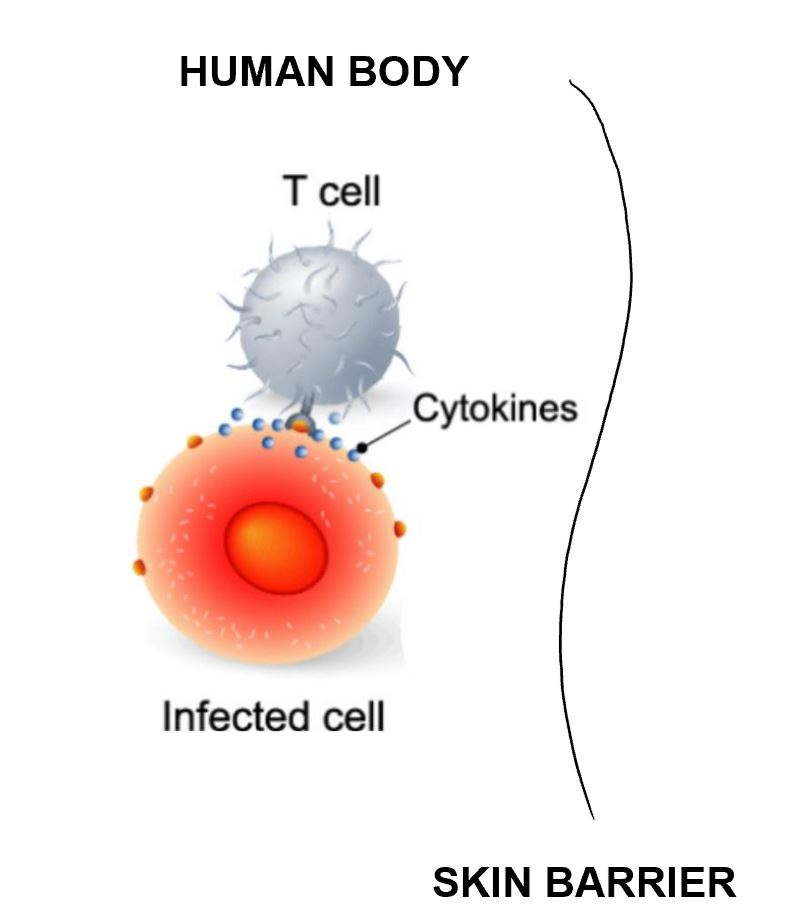
\includegraphics[width=0.5\textwidth]{physicalsys.jpg}
 }
 \caption{The Physical System}\citep{wikifig}

 \label{Fig_PhysicalSystem}
 \end{center}
 \end{figure}

\subsubsection{Goal Statements}

\noindent Given two HIV-1 viral load test datum, time duration between the tests and the chosen prediction period, the goal 
statements are:

\begin{itemize}

\item[GS\refstepcounter{goalnum}\thegoalnum 
\label{G_determine-elimination-rate}:] 
determine-elimination-rate: Determine the rate of elimination of the HIV virus 
due 
to immune response.

\item[GS\refstepcounter{goalnum}\thegoalnum \label{G_predict-VL-30}:] 
predict-VL: Predict Viral Load after chosen prediction period.

\end{itemize}

\newpage

\subsection{Solution Characteristics Specification}


The instance models that govern \progname{} are presented in
Subsection~\ref{sec_instance}.  The information to understand the meaning of the
instance models and their derivation is also presented in Assumptions, 
Theoretical Models, General Definitions and Data Definitions, so that the 
instance
models can be verified.

\subsubsection{Assumptions} \label{sec_assumpt}


This section describes the theoretical assumptions that the system will be 
based on. The theoretical models will be easier to understand by explaining 
these assumptions.

  
\begin{itemize}

\item[A\refstepcounter{assumpnum}\theassumpnum \label{initial-inf}:]
initial-inf: Initial infection of a HIV patient.

\item[A\refstepcounter{assumpnum}\theassumpnum \label{const-growth}:]
const-growth: The virions will invade uninfected cells at a constant 
rate (Ref By: \lcref{LC_more_outputs}).
  
\item[A\refstepcounter{assumpnum}\theassumpnum \label{const-volume}:]
const-volume: The dimensions of the location associated with the 
infection remains constant.(Ref By:\aref{const-conditions}, \ucref{ULC_constant-conditions})
  
\item[A\refstepcounter{assumpnum}\theassumpnum \label{const-conditions}:]
const-conditions: Temperature in the infection location remains constant. 
Higher temperatures boost virus replication and viral load \citep{10.1371/journal.ppat.1002792}. (Ref By:  
\ucref{ULC_constant-conditions})

  
\item[A\refstepcounter{assumpnum}\theassumpnum \label{all-productive}:]
all-productive: All viruses within the volume have productively infected cells. 
(Ref By: 
\ucref{ULC_constant-conditions})
  
\item[A\refstepcounter{assumpnum}\theassumpnum \label{always-elimination}:]
always-elimination: After the viremia peak, no significant upward trends occur.
   
\item[A\refstepcounter{assumpnum}\theassumpnum \label{neglect-drugs}:]
neglect-drugs: The effect of antibiotic drugs or therapy on the elimination rate 
will not be considered. (Ref By: \iref{VLelimination}, \iref{VLat30})
  
\item[A\refstepcounter{assumpnum}\theassumpnum \label{neglect-sick}:]
neglect-sick: The effect of other infections on the elimination rate will not be 
considered. (Ref By: \iref{VLelimination}, \iref{VLat30})

\item[A\refstepcounter{assumpnum}\theassumpnum \label{proportional}:]
proportional: The elimination of the virus is assumed to be proportional to the 
amount of viruses present. (Ref By: \iref{VLelimination}, \iref{VLat30})

\end{itemize}

\subsubsection{Theoretical Models}\label{sec_theoretical}

This section focuses on the general equations that \progname{} is based 
on.

~\newline

\noindent
\begin{minipage}{\textwidth}
\renewcommand*{\arraystretch}{1.5}
\begin{tabular}{| p{\colAwidth} | p{\colBwidth}|}
  \hline
  \rowcolor[gray]{0.9}
  Number& T\refstepcounter{theorynum}\thetheorynum :expElim
\label{T_expElim}\\
  \hline
  Label&\bf Rate of Change of Viral Load  \\
  \hline
  Equation&  $r$= $\frac{dN_{t}}{dt}$ = $-kN_{o}$\\
  &\\
  \hline
  Description & 
  $r$ is the rate of change of the viral load ($\frac{mol}{mLd}$)\\
  & $t$ is the time (d) \\
  & $N_t$ is the viral load at time t ($\frac{mol}{mL}$)\\
  & $k$ is the elimination constant ($d^-{1}$)\\
  & $N_o$ is the initial viral load ($\frac{mol}{mL}$)\\
  
  \hline
  Source & \citep{libretexts_2020}
\\
&\\
  \hline
  Ref.\ By & \dref{GD_vLoadt}\\ 
  \hline
\end{tabular}
\end{minipage}\\
~\newline


\subsubsection{General Definitions}\label{sec_gendef}

This section collects the laws and equations that will be used to build the 
instance models.

~\newline

\noindent
\begin{minipage}{\textwidth}
\renewcommand*{\arraystretch}{1.5}
\begin{tabular}{| p{\colAwidth} | p{\colBwidth}|}
\hline
\rowcolor[gray]{0.9}
Number& GD\refstepcounter{defnum}\thedefnum : vLoadt \label{GD_vLoadt}\\
\hline
  Label&\bf VLoadt as a function of time for constant decay rate \\
  \hline
  Equation&  $N_t$ = $N_{o} e^{-k t}$\\
  \hline
  Description &  
  $N_{o}$ is the initial amount that will undergo an exponential 
decrease. $N_{o}$ is equivalent to $N(t= 0)$.\\
&  $N_t$ is the viral load at time t ($\frac{mol}{mL}$)\\
&  $k$ is the clearing constant ($d^{-1}$) \\
&  $t$ is the time ($d$)\\

&\\
\hline
  Source & \citep{hobbie_roth_1970}
 \\
  \hline
  Ref.\ By & \iref{VLelimination} , \iref{VLat30}\\
  \hline
\end{tabular}
\end{minipage}\\

\subsubsection*{Detailed derivation of viral load at time t:}

\label{GD:vLoadtDeriv}
Using the First-Order rate Law in \hyperref[T_expElim]{TM: expElim}, we have:

\begin{displaymath}
\frac{\,dN}{\,dt}=-k {N_{\text{o}}}
\end{displaymath}
Where ${N_{\text{t}}}$ denotes the viral load at time t, ${N_{\text{o}}}$ 
denotes the initial viral load and $k$ denotes the elimination constant. When 
rearranging for integration,  we have:

\begin{displaymath}
\int_{{N_{\text{o}}}}^{{N_{\text{t}}}}{1}\,d{N_{\text{t}}}=-\int_{0}^{t}{k}\,dt
\end{displaymath}
Performing the integration, we have the required equation:

\begin{displaymath}
{N_{\text{t}}}={N_{\text{o}}} e^{-k t}
\end{displaymath}



\subsubsection{Data Definitions}\label{sec_datadef}

This section collects and defines all the data needed to build the instance 
models.
 
~\newline

\noindent
\begin{minipage}{\textwidth}
\renewcommand*{\arraystretch}{1.5}
\begin{tabular}{| p{\colAwidth} | p{\colBwidth}|}
\hline
\rowcolor[gray]{0.9}
Number& DD\refstepcounter{datadefnum}\thedatadefnum: Viral load
\label{DD_viralload}\\
\hline
Label& \bf Viral Load \\
\hline
Symbol &$N$\\
\hline

&\\
  Units & $\dfrac{mol}{mL}$\\
  &\\
  \hline
  &\\
  Equation& $N = \dfrac{n}{V}$ \\
  &\\
  \hline
  Description & 
 $N$ is the viral load at a given time ($\dfrac{mol}{mL}$). \\
 & $n$ is the number of virions ($mol$).\\
 & $V$ is the volume ($mL$).\\
&\\
  \hline
  Sources& \citep{Fischer6706}
 \\
  \hline
  Ref.\ By & \iref{VLelimination} , \iref{VLat30}\\
  \hline
\end{tabular}
\end{minipage}\\

\subsubsection{Instance Models} \label{sec_instance}    

This section transforms the problem defined in Section~\ref{Sec_pd} into one 
which is expressed in mathematical terms. It uses concrete symbols defined in 
Section~\ref{sec_datadef} to replace the abstract symbols in the models 
identified in Sections~\ref{sec_theoretical} and~\ref{sec_gendef}.

The goals GS\ref{G_determine-elimination-rate}: determine-elimination-rate and 
GS\ref{G_predict-VL-30}: predict-VL-30 are met by \iref{VLelimination}and \iref{VLat30}.



~\newline

%Instance Model 1

\noindent
\begin{minipage}{\textwidth}
\renewcommand*{\arraystretch}{1.5}
\begin{tabular}{| p{\colAwidth} | p{\colBwidth}|}
  \hline
  \rowcolor[gray]{0.9}
  Number& IM\refstepcounter{instnum}\theinstnum : calofElimConst 
\label{VLelimination}\\
  \hline
  Label& \bf Calculation of elimination rate\\
  \hline
  Input&$N_{t}$, $N_{o}$, $t_{t}$\\
  & The input is constrained so that $N_{o} > N_{t} > 0$, $t_{t} > 0$
\\
  \hline  
  Output& $ k$, such that\\
  &$k = \frac{ln(N_{o})-ln(N_{t})}{t_{t}}$\\
 
  \hline
  Description
  & $k$ is the elimination constant ($d^{-1}$)\\
  & $N_{o}$ is the initial viral load ($\frac{mol}{mL}$)\\
  & $N_t$ is the viral load at time t ($\frac{mol}{mL}$)\\
  &  $t_{t}$ is the time duration between the initial viral load test and 
secondary viral load test ($d$)\\
  
  \hline
  Sources& \citep{libretexts_2020}

\\
  \\
  \hline
  Ref.\ By & \iref{VLat30} \\
  \hline
\end{tabular}
\end{minipage}\\

%~\newline
\subsubsection*{Detailed derivation of elimination constant:}
\label{IM:calofElimConstDeriv}
Using the relationship for the viral load seen in \hyperref[DD_viralload]{DD: 
viralLoad} with respect to time in \hyperref[GD_vLoadt]{GD: vLoadt}, we have:

\begin{displaymath}
{N_{\text{t}}}={N_{\text{o}}} e^{-k {t_{\text{t}}}}
\end{displaymath}
Where ${N_{\text{t}}}$ denotes the viral load at time $t_{\text{t}}$, ${N_{\text{o}}}$ 
denotes the initial viral load and $k$ denotes the elimination constant. When 
isolating for the elimination constant,  we have:

\begin{displaymath}
\frac{{N_{\text{t}}}}{{N_{\text{o}}}}=e^{-k {t_{\text{t}}}}
\end{displaymath}
To isolate further, the natural logarithm is applied:

\begin{displaymath}
\ln\left(\frac{{N_{\text{t}}}}{{N_{\text{o}}}}\right)=-k {t_{\text{t}}}
\end{displaymath}
After using the logarithmic quotient property, we have the required equation:

\begin{displaymath}
k=\frac{\ln\left({N_{\text{o}}}\right)-\ln\left({N_{\text{t}}}\right)}{{t_{\text{t}}}}
\end{displaymath}

  
~\newline
%Instance Model 2

\noindent
\begin{minipage}{\textwidth}
\renewcommand*{\arraystretch}{1.5}
\begin{tabular}{| p{\colAwidth} | p{\colBwidth}|}
  \hline
  \rowcolor[gray]{0.9}
  Number& IM\refstepcounter{instnum}\theinstnum : calofPredictedVL 
\label{VLat30}\\
  \hline
  Label& \bf Calculation of predicted viral load
 \\
  \hline
  Input
  & $N_{o}$, $k$, $t_{p}$ from \iref{VLelimination}\\
  & The input is constrained so that $N_{o} > N_{t} > 0$, $t_{p} > t_{t} > 0$ 
and $k > 0$
 \\
  \hline
  Output
  & $N_p$, such that\\
  & $N_p$ = $N_{o} e^{-k t_{p}}$\\
   \\
  \hline
  Description
&  $N_p$ is the predicted viral load after 30 days ($\frac{mol}{mL}$)\\
&  $N_{o}$ is the initial viral load ($\frac{mol}{mL}$)\\
&  $k$ is the clearing constant ($d^{-1}$) \\
&  $t_p$ is the chosen prediction period ($d$)\\
  \\
  \hline
  Sources& \citep{hobbie_roth_1970}
  \\
  \hline
  Ref.\ By & -\\
  \hline
\end{tabular}
\end{minipage}\\

\subsubsection*{Detailed derivation of predicted viral load after 30 days:}

\label{IM:calofPredictedVLDeriv}
Using the relationship for the viral load seen in \hyperref[DD_viralload]{DD: 
viralLoad} with respect to time in \hyperref[GD_vLoadt]{GD: vLoadt}, we have:

\begin{displaymath}
{N_{\text{t}}}={N_{\text{o}}} e^{-k {t_{\text{t}}}}
\end{displaymath}
Where ${N_{\text{t}}}$ denotes the viral load at time t, ${N_{\text{o}}}$ 
denotes the initial viral load and $k$ denotes the elimination constant. When 
predicting the viral load after 30 days, the elimination constant  found in 
\hyperref[VLelimination]{IM: calofElimConst},  is used instead of 
${N_{\text{t}}}$  therefore we have:

\begin{displaymath}
{N_{\text{p}}}={N_{\text{o}}} e^{-k {t_{\text{p}}}}
\end{displaymath}

%~\newline


\subsubsection{Input Data Constraints} \label{sec_DataConstraints}    

Table~\ref{TblInputVar} shows the data constraints on the input 
variables.  The column for physical constraints gives the physical limitations
on the range of values that can be taken by the variable.  The column for
software constraints restricts the range of inputs to reasonable values.  The
software constraints will be helpful in the design stage for picking suitable
algorithms.  The constraints are conservative, to give the user of the model the
flexibility to experiment with unusual situations.  The column of typical values
is intended to provide a feel for a common scenario.  The uncertainty column
provides an estimate of the confidence with which the physical quantities can be
measured.  This information would be part of the input if one were performing an
uncertainty quantification exercise.

\begin{center}

\begin{table}[!h]
  \caption{Input Variables} \label{TblInputVar}
  \renewcommand{\arraystretch}{1.2}
\noindent \begin{longtable*}{l l l l c} 
  \toprule
  \textbf{Var} & \textbf{Physical Constraints} & \textbf{Software Constraints} &
                             \textbf{Typical Value} & \textbf{Uncertainty}\\
  \midrule 
  $N_o$ & $N_o > 0$ & $N_o > N_t $ & $10*10^6 \frac{mol}{mL}$ & 
10\%\\
  $N_t$ & $N_t > 0$ & $N_o > N_t > 0$ & $5*10^6 \frac{mol}{mL}$ & 10\%\\
  $t_{p}$ &  $t_{p} > 0$ &  $t_{p}> t_{t} $ & 30 d & N/A\\
  $t_{t}$ &  $t_{p} > t_{t} > 0$ &  $t_{p}> t_{t} $ & 1 d & N/A\\
  \\
  \bottomrule
\end{longtable*}
\end{table}

\end{center}


\subsubsection{Properties of a Correct Solution} \label{sec_CorrectSolution}

\noindent
A correct solution must exhibit an elimination constant greater than 0 and a predicted viral load less than the initial and secondary viral load, $N_o$ and $N_t$, respectively. 
Table~\ref{TblOutputVar} shows the data constraints for the output variables. 


\begin{table}[!h]
\caption{Output Variables} \label{TblOutputVar}
\renewcommand{\arraystretch}{1.2}
\noindent \begin{longtable*}{l l} 
  \toprule
  \textbf{Var} & \textbf{Physical Constraints} \\
  \midrule 
  $k$ & $k > 0 $ 
  \\ 
  $N_p$ & $N_o > N_p > 0 $ 
   \\
  \bottomrule
\end{longtable*}
\end{table}

~\newpage
\section{Requirements}

This section provides the functional requirements, the business tasks that the
software is expected to complete, and the non-functional requirements, the
qualities that the software is expected to exhibit.

\subsection{Functional Requirements}
\label{sec_FunctionalReq}

\noindent \begin{itemize}

\item[R\refstepcounter{reqnum}\thereqnum \label{R_Inputs}:]Input-Values: Input 
the values from subsection
 \ref{sec_DataConstraints}.

\item[R\refstepcounter{reqnum}\thereqnum \label{R_VerifyInputs}:] 
Verify-Input-Values: The software will ensure that the inputs are not out of 
bounds and in accordance with the data constraints. If any inputs are out of 
bounds, an error message is displayed in subsection \ref{sec_DataConstraints}.
    
\item[R\refstepcounter{reqnum}\thereqnum \label{R_Calculate}:] 
Calculate-Values: Software calculates the elimination rate of HIV and the viral 
load at the chosen prediction period from \iref{VLelimination} and 
\iref{VLat30}.

\item[R\refstepcounter{reqnum}\thereqnum \label{R_VerifyOutput}:]
Verify-Output: The output values will be cross referenced with the result 
constraints from subsection \ref{sec_CorrectSolution}.

\item[R\refstepcounter{reqnum}\thereqnum \label{R_Output}:] 
Output-Values: Output related requirements including the elimination rate and 
predicted viral load.

\end{itemize}


\subsection{Non-functional Requirements}

This section provides the non-functional requirements, the qualities that the 
software is expected to exhibit.

\noindent \begin{itemize}

\item[NR\refstepcounter{nreqnum}\thenreqnum \label{NR_Verifiable}:] 
Verifiable: The Drasil generated python code is tested using static and dynamic 
code analysis, linting, unit and system testing and continuous integration 
methods outlined in the Verification and Validation plan of Diagnose 
\citep{DiagnoseVNVplan}.


\item[NR\refstepcounter{nreqnum}\thenreqnum \label{NR_Understandability}:] 
Understandability: The code will be generated using the Drasil Framework into 
modules to address each requirement in subsection \ref{sec_FunctionalReq}.

\item[NR\refstepcounter{nreqnum}\thenreqnum \label{NR_Reusable}:] 
Reusable: The code will be created using Drasil. The framework has data 
libraries of scientific theories, concepts, quantities and units commonly used 
in scientific problems. The created libraries of \progname{} can be reused as 
required. \citep{Drasilcreate}

\item[NR\refstepcounter{nreqnum}\thenreqnum \label{NR_Maintainability}:] 
Maintainablility: The traceability between requirements, assumptions, 
theoretical models, general 
definitions, data definitions, instance models, likely changes, unlikely 
changes, and modules is completely recorded in traceability matrices in the SRS 
document to measure maintainability. The traceability will be measured by 
ensuring relationship from inputs to instance model is recorded and 
identifiable.

\item[NR\refstepcounter{nreqnum}\thenreqnum \label{NR_Portablility}:] 
Portablility: The generated code is able to run in different environments. 


\end{itemize}


\section{Likely Changes} 

This section lists the likely changes to be made to software   

\noindent \begin{itemize}

\item[LC\refstepcounter{lcnum}\thelcnum\label{LC_more_inputs}:] More-Inputs: The 
software may be expanded to include more inputs from the user to increase the 
accuracy of the output.

\item[LC\refstepcounter{lcnum}\thelcnum\label{LC_more_outputs}:] 
More-outputs: The program may be extended to include more outputs like assessing 
the progression to AIDs or suggestion for therapy.
\end{itemize}

\section{Unlikely Changes}    

This section lists the unlikely changes to be made to the software.

\begin{itemize}

\item[UC\refstepcounter{ucnum}\theucnum\label{ULC_determine-elimination-rate}:] 
determine-elimination-rate: The goal of determining the elimination rate of the 
virus will not likely change.

\item[UC\refstepcounter{ucnum}\theucnum\label{ULC_external-input}:] 
external-input: There will always be a source of input data external to the 
software.

\item[UC\refstepcounter{ucnum}\theucnum\label{ULC_constant-conditions}:] 
constant-conditions: The input constraints will not likely change.
\end{itemize}

\section{Traceability Matrices and Graphs}

The purpose of the traceability matrices is to provide easy references on what
has to be additionally modified if a certain component is changed.  Every time a
component is changed, the items in the column of that component that are marked
with an ``X'' may have to be modified as well.  Table~\ref{Table:trace} shows 
the
dependencies of theoretical models, general definitions, data definitions, and
instance models with each other. Table~\ref{Table:R_trace} shows the
dependencies of instance models, requirements, and data constraints on each
other. Table~\ref{Table:A_trace} shows the dependencies of theoretical models,
general definitions, data definitions, instance models, and likely changes on
the assumptions.


\afterpage{
%\begin{landscape}
\begin{table}[h!]
\centering
\begin{tabular}{|c|c|c|c|c|c|c|c|c|c|}
\hline
	& \aref{initial-inf}& \aref{const-growth}& \aref{const-volume}& 
\aref{const-conditions}& 
\aref{all-productive}& \aref{always-elimination}& \aref{neglect-drugs}& 
\aref{neglect-sick}& \aref{proportional} \\
\hline
\tref{T_expElim}        &X & & & & &X & & &  \\ \hline
\dref{GD_vLoadt}           & &X &X &X & & & & &X  \\ \hline
\ddref{DD_viralload}     & &X &X &X &X & & & &X  \\ \hline
\iref{VLelimination}         & &X &X &X &X & & & &X  \\ \hline
\iref{VLat30}         & &X &X &X &X &X & & &X  \\ \hline
\lcref{LC_more_inputs}     &X & & & & & & & &  \\ \hline
\lcref{LC_more_outputs}    & & & & &X &X & & &X  \\ \hline

\hline
\end{tabular}
\caption{Traceability Matrix Showing the Connections Between Assumptions and 
Other Items}

\label{Table:A_trace}
\end{table}
%\end{landscape}
}

\begin{table}[h!]
\centering
\begin{tabular}{|c|c|c|c|c|c|c|}
\hline        
	& \tref{T_expElim}&  \dref{GD_vLoadt}& \ddref{DD_viralload}& 
\iref{VLelimination} & 
\iref{VLat30} \\
\hline
\tref{T_expElim}        & & & & &  \\ \hline
\dref{GD_vLoadt}        & & & & &  \\ \hline
\ddref{DD_viralload}    & &X & & &  \\ \hline
\iref{VLelimination}    &X & &X & &X  \\ \hline
\iref{VLat30}           &X & &X &X & \\ 
\hline
\end{tabular}
\caption{Traceability Matrix Showing the Connections Between Items of Different 
Sections}
\label{Table:trace}
\end{table}

\begin{table}[h!]
\centering
\begin{tabular}{|c|c|c|c|c|c|c|}
\hline
	& \ref{sec_DataConstraints}& \rref{R_Inputs}& 
\rref{R_VerifyInputs}& \rref{R_Calculate}& 
\rref{R_VerifyOutput}& \rref{R_Output} 
\\
\hline
\iref{VLelimination}    &X & & &X &X &X \\ \hline
\iref{VLat30}		   &X & & &X &X &X  \\ 
\hline
\end{tabular}
\caption{Traceability Matrix Showing the Connections Between Requirements and 
Instance Models}
\label{Table:R_trace}
\end{table}

The purpose of the traceability graphs is also to provide easy references on
what has to be additionally modified if a certain component is changed.  The
arrows in the graphs represent dependencies. The component at the tail of an
arrow is depended on by the component at the head of that arrow. Therefore, if a
component is changed, the components that it points to should also be
changed. 


\newpage

\section{References}

\bibliographystyle{plainnat}
\bibliography{references.bib}

%\newpage

%\bibliographystyle {plainnat}
%\bibliography {../../refs/References}


\newpage

\newpage


\end{document}

